% Created by tikzDevice version 0.12.3 on 2020-12-22 01:51:53
% !TEX encoding = UTF-8 Unicode
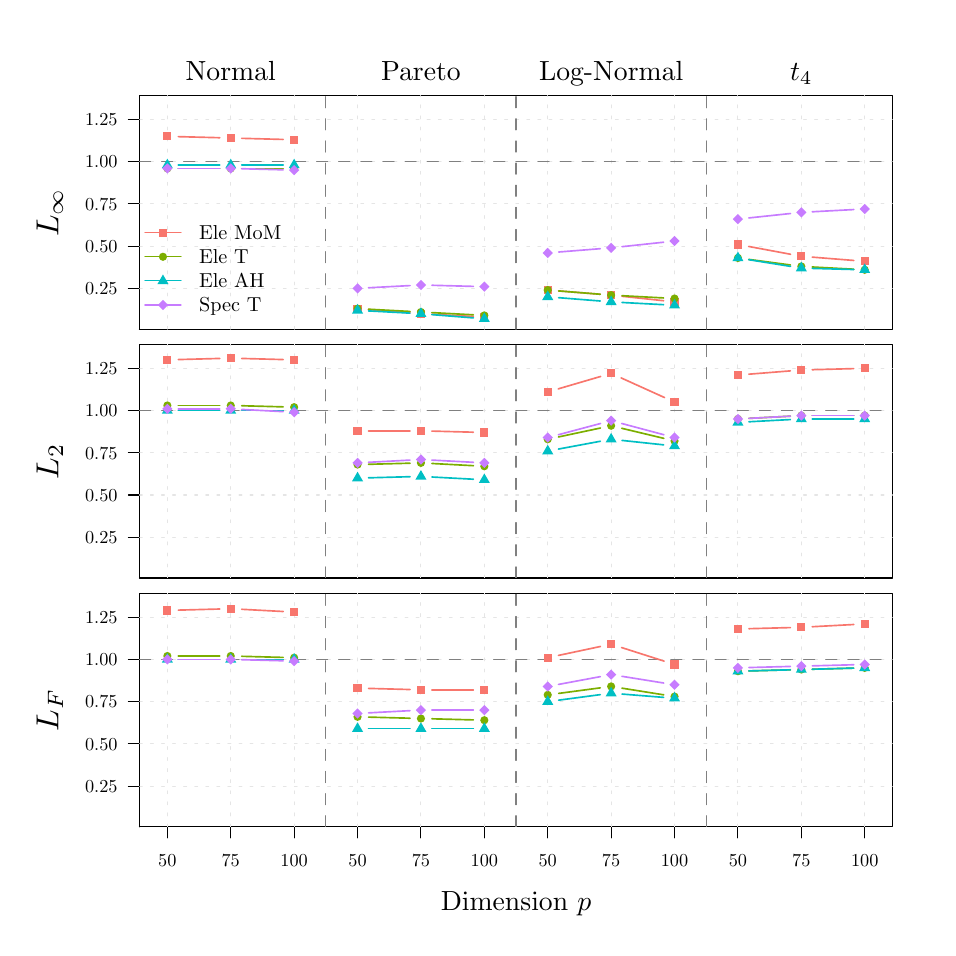
\begin{tikzpicture}[x=1pt,y=1pt]
\definecolor{fillColor}{RGB}{255,255,255}
\path[use as bounding box,fill=fillColor,fill opacity=0.00] (0,0) rectangle (325.21,325.21);
\begin{scope}
\path[clip] (  0.00,  0.00) rectangle (325.21,325.21);
\definecolor{drawColor}{RGB}{0,0,0}

\path[draw=drawColor,line width= 0.4pt,line join=round,line cap=round] ( 40.39,216.28) --
	(312.54,216.28) --
	(312.54,300.66) --
	( 40.39,300.66) --
	( 40.39,216.28);

\path[draw=drawColor,line width= 0.4pt,line join=round,line cap=round] ( 40.39,231.00) -- ( 40.39,292.04);

\path[draw=drawColor,line width= 0.4pt,line join=round,line cap=round] ( 40.39,231.00) -- ( 36.43,231.00);

\path[draw=drawColor,line width= 0.4pt,line join=round,line cap=round] ( 40.39,246.26) -- ( 36.43,246.26);

\path[draw=drawColor,line width= 0.4pt,line join=round,line cap=round] ( 40.39,261.52) -- ( 36.43,261.52);

\path[draw=drawColor,line width= 0.4pt,line join=round,line cap=round] ( 40.39,276.78) -- ( 36.43,276.78);

\path[draw=drawColor,line width= 0.4pt,line join=round,line cap=round] ( 40.39,292.04) -- ( 36.43,292.04);

\node[text=drawColor,anchor=base east,inner sep=0pt, outer sep=0pt, scale=  0.66] at ( 32.47,228.73) {0.25};

\node[text=drawColor,anchor=base east,inner sep=0pt, outer sep=0pt, scale=  0.66] at ( 32.47,243.99) {0.50};

\node[text=drawColor,anchor=base east,inner sep=0pt, outer sep=0pt, scale=  0.66] at ( 32.47,259.25) {0.75};

\node[text=drawColor,anchor=base east,inner sep=0pt, outer sep=0pt, scale=  0.66] at ( 32.47,274.51) {1.00};

\node[text=drawColor,anchor=base east,inner sep=0pt, outer sep=0pt, scale=  0.66] at ( 32.47,289.77) {1.25};
\end{scope}
\begin{scope}
\path[clip] ( 40.39,216.28) rectangle (312.54,300.66);
\definecolor{drawColor}{gray}{0.90}

\path[draw=drawColor,line width= 0.4pt,dash pattern=on 1pt off 3pt ,line join=round,line cap=round] ( 40.39,231.00) -- (312.54,231.00);

\path[draw=drawColor,line width= 0.4pt,dash pattern=on 1pt off 3pt ,line join=round,line cap=round] ( 40.39,246.26) -- (312.54,246.26);

\path[draw=drawColor,line width= 0.4pt,dash pattern=on 1pt off 3pt ,line join=round,line cap=round] ( 40.39,261.52) -- (312.54,261.52);

\path[draw=drawColor,line width= 0.4pt,dash pattern=on 1pt off 3pt ,line join=round,line cap=round] ( 40.39,276.78) -- (312.54,276.78);

\path[draw=drawColor,line width= 0.4pt,dash pattern=on 1pt off 3pt ,line join=round,line cap=round] ( 40.39,292.04) -- (312.54,292.04);

\path[draw=drawColor,line width= 0.4pt,dash pattern=on 1pt off 3pt ,line join=round,line cap=round] ( 50.47,216.28) -- ( 50.47,300.66);

\path[draw=drawColor,line width= 0.4pt,dash pattern=on 1pt off 3pt ,line join=round,line cap=round] ( 73.38,216.28) -- ( 73.38,300.66);

\path[draw=drawColor,line width= 0.4pt,dash pattern=on 1pt off 3pt ,line join=round,line cap=round] ( 96.29,216.28) -- ( 96.29,300.66);

\path[draw=drawColor,line width= 0.4pt,dash pattern=on 1pt off 3pt ,line join=round,line cap=round] (119.20,216.28) -- (119.20,300.66);

\path[draw=drawColor,line width= 0.4pt,dash pattern=on 1pt off 3pt ,line join=round,line cap=round] (142.10,216.28) -- (142.10,300.66);

\path[draw=drawColor,line width= 0.4pt,dash pattern=on 1pt off 3pt ,line join=round,line cap=round] (165.01,216.28) -- (165.01,300.66);

\path[draw=drawColor,line width= 0.4pt,dash pattern=on 1pt off 3pt ,line join=round,line cap=round] (187.92,216.28) -- (187.92,300.66);

\path[draw=drawColor,line width= 0.4pt,dash pattern=on 1pt off 3pt ,line join=round,line cap=round] (210.83,216.28) -- (210.83,300.66);

\path[draw=drawColor,line width= 0.4pt,dash pattern=on 1pt off 3pt ,line join=round,line cap=round] (233.74,216.28) -- (233.74,300.66);

\path[draw=drawColor,line width= 0.4pt,dash pattern=on 1pt off 3pt ,line join=round,line cap=round] (256.65,216.28) -- (256.65,300.66);

\path[draw=drawColor,line width= 0.4pt,dash pattern=on 1pt off 3pt ,line join=round,line cap=round] (279.56,216.28) -- (279.56,300.66);

\path[draw=drawColor,line width= 0.4pt,dash pattern=on 1pt off 3pt ,line join=round,line cap=round] (302.46,216.28) -- (302.46,300.66);
\definecolor{drawColor}{gray}{0.50}

\path[draw=drawColor,line width= 0.4pt,dash pattern=on 4pt off 4pt ,line join=round,line cap=round] (107.74,216.28) -- (107.74,300.66);

\path[draw=drawColor,line width= 0.4pt,dash pattern=on 4pt off 4pt ,line join=round,line cap=round] (176.47,216.28) -- (176.47,300.66);

\path[draw=drawColor,line width= 0.4pt,dash pattern=on 4pt off 4pt ,line join=round,line cap=round] (245.19,216.28) -- (245.19,300.66);

\path[draw=drawColor,line width= 0.4pt,dash pattern=on 4pt off 4pt ,line join=round,line cap=round] (313.92,216.28) -- (313.92,300.66);
\end{scope}
\begin{scope}
\path[clip] (  0.00,  0.00) rectangle (325.21,325.21);
\definecolor{drawColor}{RGB}{0,0,0}

\node[text=drawColor,rotate= 90.00,anchor=base,inner sep=0pt, outer sep=0pt, scale=  1.15] at ( 11.09,258.47) {$L_{\infty}$};
\end{scope}
\begin{scope}
\path[clip] ( 40.39,216.28) rectangle (312.54,300.66);
\definecolor{drawColor}{gray}{0.50}

\path[draw=drawColor,line width= 0.4pt,dash pattern=on 4pt off 4pt ,line join=round,line cap=round] ( 40.39,276.78) -- (312.54,276.78);
\end{scope}
\begin{scope}
\path[clip] (  0.00,  0.00) rectangle (325.21,325.21);
\definecolor{drawColor}{RGB}{0,0,0}

\node[text=drawColor,anchor=base,inner sep=0pt, outer sep=0pt, scale=  1.00] at ( 73.38,306.21) {Normal};

\node[text=drawColor,anchor=base,inner sep=0pt, outer sep=0pt, scale=  1.00] at (142.10,306.21) {Pareto};

\node[text=drawColor,anchor=base,inner sep=0pt, outer sep=0pt, scale=  1.00] at (210.83,306.21) {Log-Normal};

\node[text=drawColor,anchor=base,inner sep=0pt, outer sep=0pt, scale=  1.00] at (279.56,306.21) {$t_4$};
\end{scope}
\begin{scope}
\path[clip] ( 40.39,216.28) rectangle (312.54,300.66);
\definecolor{drawColor}{RGB}{248,118,109}

\path[draw=drawColor,line width= 0.4pt,line join=round,line cap=round] ( 42.35,251.13) -- ( 55.42,251.13);
\definecolor{drawColor}{RGB}{124,174,0}

\path[draw=drawColor,line width= 0.4pt,line join=round,line cap=round] ( 42.35,242.42) -- ( 55.42,242.42);
\definecolor{drawColor}{RGB}{0,191,196}

\path[draw=drawColor,line width= 0.4pt,line join=round,line cap=round] ( 42.35,233.71) -- ( 55.42,233.71);
\definecolor{drawColor}{RGB}{199,124,255}

\path[draw=drawColor,line width= 0.4pt,line join=round,line cap=round] ( 42.35,224.99) -- ( 55.42,224.99);
\definecolor{fillColor}{RGB}{248,118,109}

\path[fill=fillColor] ( 47.40,249.64) --
	( 50.37,249.64) --
	( 50.37,252.61) --
	( 47.40,252.61) --
	cycle;
\definecolor{fillColor}{RGB}{124,174,0}

\path[fill=fillColor] ( 48.89,242.42) circle (  1.48);
\definecolor{fillColor}{RGB}{0,191,196}

\path[fill=fillColor] ( 48.89,236.02) --
	( 50.89,232.55) --
	( 46.89,232.55) --
	cycle;
\definecolor{fillColor}{RGB}{199,124,255}

\path[fill=fillColor] ( 47.03,224.99) --
	( 48.89,226.85) --
	( 50.74,224.99) --
	( 48.89,223.14) --
	cycle;
\definecolor{drawColor}{RGB}{0,0,0}

\node[text=drawColor,anchor=base west,inner sep=0pt, outer sep=0pt, scale=  0.73] at ( 61.95,248.63) {Ele MoM};

\node[text=drawColor,anchor=base west,inner sep=0pt, outer sep=0pt, scale=  0.73] at ( 61.95,239.92) {Ele T};

\node[text=drawColor,anchor=base west,inner sep=0pt, outer sep=0pt, scale=  0.73] at ( 61.95,231.21) {Ele AH};

\node[text=drawColor,anchor=base west,inner sep=0pt, outer sep=0pt, scale=  0.73] at ( 61.95,222.49) {Spec T};
\definecolor{drawColor}{RGB}{248,118,109}

\path[draw=drawColor,line width= 0.6pt,line join=round,line cap=round] ( 54.43,285.83) -- ( 69.42,285.44);

\path[draw=drawColor,line width= 0.6pt,line join=round,line cap=round] ( 77.34,285.22) -- ( 92.33,284.82);
\definecolor{fillColor}{RGB}{248,118,109}

\path[fill=fillColor] ( 48.99,284.46) --
	( 51.96,284.46) --
	( 51.96,287.43) --
	( 48.99,287.43) --
	cycle;

\path[fill=fillColor] ( 71.89,283.84) --
	( 74.86,283.84) --
	( 74.86,286.81) --
	( 71.89,286.81) --
	cycle;

\path[fill=fillColor] ( 94.80,283.23) --
	( 97.77,283.23) --
	( 97.77,286.20) --
	( 94.80,286.20) --
	cycle;
\definecolor{drawColor}{RGB}{124,174,0}

\path[draw=drawColor,line width= 0.6pt,line join=round,line cap=round] ( 54.43,274.34) -- ( 69.42,274.34);

\path[draw=drawColor,line width= 0.6pt,line join=round,line cap=round] ( 77.34,274.34) -- ( 92.33,274.34);
\definecolor{fillColor}{RGB}{124,174,0}

\path[fill=fillColor] ( 50.47,274.34) circle (  1.48);

\path[fill=fillColor] ( 73.38,274.34) circle (  1.48);

\path[fill=fillColor] ( 96.29,274.34) circle (  1.48);
\definecolor{drawColor}{RGB}{0,191,196}

\path[draw=drawColor,line width= 0.6pt,line join=round,line cap=round] ( 54.43,275.56) -- ( 69.42,275.56);

\path[draw=drawColor,line width= 0.6pt,line join=round,line cap=round] ( 77.34,275.56) -- ( 92.33,275.56);
\definecolor{fillColor}{RGB}{0,191,196}

\path[fill=fillColor] ( 50.47,277.87) --
	( 52.47,274.41) --
	( 48.47,274.41) --
	cycle;

\path[fill=fillColor] ( 73.38,277.87) --
	( 75.38,274.41) --
	( 71.38,274.41) --
	cycle;

\path[fill=fillColor] ( 96.29,277.87) --
	( 98.29,274.41) --
	( 94.29,274.41) --
	cycle;
\definecolor{drawColor}{RGB}{199,124,255}

\path[draw=drawColor,line width= 0.6pt,line join=round,line cap=round] ( 54.43,274.34) -- ( 69.42,274.34);

\path[draw=drawColor,line width= 0.6pt,line join=round,line cap=round] ( 77.34,274.24) -- ( 92.33,273.84);
\definecolor{fillColor}{RGB}{199,124,255}

\path[fill=fillColor] ( 48.62,274.34) --
	( 50.47,276.20) --
	( 52.33,274.34) --
	( 50.47,272.49) --
	cycle;

\path[fill=fillColor] ( 71.52,274.34) --
	( 73.38,276.20) --
	( 75.24,274.34) --
	( 73.38,272.49) --
	cycle;

\path[fill=fillColor] ( 94.43,273.73) --
	( 96.29,275.59) --
	( 98.14,273.73) --
	( 96.29,271.88) --
	cycle;
\definecolor{drawColor}{RGB}{248,118,109}

\path[draw=drawColor,line width= 0.6pt,line join=round,line cap=round] (123.14,223.36) -- (138.16,222.16);

\path[draw=drawColor,line width= 0.6pt,line join=round,line cap=round] (146.06,221.64) -- (161.06,220.84);
\definecolor{fillColor}{RGB}{248,118,109}

\path[fill=fillColor] (117.71,222.19) --
	(120.68,222.19) --
	(120.68,225.16) --
	(117.71,225.16) --
	cycle;

\path[fill=fillColor] (140.62,220.36) --
	(143.59,220.36) --
	(143.59,223.33) --
	(140.62,223.33) --
	cycle;

\path[fill=fillColor] (163.53,219.14) --
	(166.50,219.14) --
	(166.50,222.11) --
	(163.53,222.11) --
	cycle;
\definecolor{drawColor}{RGB}{124,174,0}

\path[draw=drawColor,line width= 0.6pt,line join=round,line cap=round] (123.15,223.47) -- (138.15,222.67);

\path[draw=drawColor,line width= 0.6pt,line join=round,line cap=round] (146.06,222.25) -- (161.06,221.45);
\definecolor{fillColor}{RGB}{124,174,0}

\path[fill=fillColor] (119.20,223.68) circle (  1.48);

\path[fill=fillColor] (142.10,222.46) circle (  1.48);

\path[fill=fillColor] (165.01,221.24) circle (  1.48);
\definecolor{drawColor}{RGB}{0,191,196}

\path[draw=drawColor,line width= 0.6pt,line join=round,line cap=round] (123.15,222.86) -- (138.15,222.06);

\path[draw=drawColor,line width= 0.6pt,line join=round,line cap=round] (146.05,221.53) -- (161.07,220.33);
\definecolor{fillColor}{RGB}{0,191,196}

\path[fill=fillColor] (119.20,225.38) --
	(121.20,221.91) --
	(117.20,221.91) --
	cycle;

\path[fill=fillColor] (142.10,224.16) --
	(144.10,220.69) --
	(140.11,220.69) --
	cycle;

\path[fill=fillColor] (165.01,222.33) --
	(167.01,218.86) --
	(163.01,218.86) --
	cycle;
\definecolor{drawColor}{RGB}{199,124,255}

\path[draw=drawColor,line width= 0.6pt,line join=round,line cap=round] (123.15,231.22) -- (138.15,232.01);

\path[draw=drawColor,line width= 0.6pt,line join=round,line cap=round] (146.06,232.12) -- (161.05,231.72);
\definecolor{fillColor}{RGB}{199,124,255}

\path[fill=fillColor] (117.34,231.00) --
	(119.20,232.86) --
	(121.05,231.00) --
	(119.20,229.15) --
	cycle;

\path[fill=fillColor] (140.25,232.23) --
	(142.10,234.08) --
	(143.96,232.23) --
	(142.10,230.37) --
	cycle;

\path[fill=fillColor] (163.16,231.62) --
	(165.01,233.47) --
	(166.87,231.62) --
	(165.01,229.76) --
	cycle;
\definecolor{drawColor}{RGB}{248,118,109}

\path[draw=drawColor,line width= 0.6pt,line join=round,line cap=round] (191.87,230.08) -- (206.88,228.88);

\path[draw=drawColor,line width= 0.6pt,line join=round,line cap=round] (214.77,228.14) -- (229.80,226.54);
\definecolor{fillColor}{RGB}{248,118,109}

\path[fill=fillColor] (186.44,228.91) --
	(189.41,228.91) --
	(189.41,231.88) --
	(186.44,231.88) --
	cycle;

\path[fill=fillColor] (209.34,227.08) --
	(212.31,227.08) --
	(212.31,230.05) --
	(209.34,230.05) --
	cycle;

\path[fill=fillColor] (232.25,224.64) --
	(235.22,224.64) --
	(235.22,227.61) --
	(232.25,227.61) --
	cycle;
\definecolor{drawColor}{RGB}{124,174,0}

\path[draw=drawColor,line width= 0.6pt,line join=round,line cap=round] (191.87,230.08) -- (206.88,228.88);

\path[draw=drawColor,line width= 0.6pt,line join=round,line cap=round] (214.78,228.35) -- (229.78,227.55);
\definecolor{fillColor}{RGB}{124,174,0}

\path[fill=fillColor] (187.92,230.39) circle (  1.48);

\path[fill=fillColor] (210.83,228.56) circle (  1.48);

\path[fill=fillColor] (233.74,227.34) circle (  1.48);
\definecolor{drawColor}{RGB}{0,191,196}

\path[draw=drawColor,line width= 0.6pt,line join=round,line cap=round] (191.87,227.64) -- (206.88,226.44);

\path[draw=drawColor,line width= 0.6pt,line join=round,line cap=round] (214.78,225.91) -- (229.78,225.11);
\definecolor{fillColor}{RGB}{0,191,196}

\path[fill=fillColor] (187.92,230.26) --
	(189.92,226.80) --
	(185.92,226.80) --
	cycle;

\path[fill=fillColor] (210.83,228.43) --
	(212.83,224.97) --
	(208.83,224.97) --
	cycle;

\path[fill=fillColor] (233.74,227.21) --
	(235.74,223.75) --
	(231.74,223.75) --
	cycle;
\definecolor{drawColor}{RGB}{199,124,255}

\path[draw=drawColor,line width= 0.6pt,line join=round,line cap=round] (191.87,244.14) -- (206.88,245.34);

\path[draw=drawColor,line width= 0.6pt,line join=round,line cap=round] (214.77,246.07) -- (229.80,247.68);
\definecolor{fillColor}{RGB}{199,124,255}

\path[fill=fillColor] (186.07,243.82) --
	(187.92,245.68) --
	(189.78,243.82) --
	(187.92,241.97) --
	cycle;

\path[fill=fillColor] (208.97,245.65) --
	(210.83,247.51) --
	(212.69,245.65) --
	(210.83,243.80) --
	cycle;

\path[fill=fillColor] (231.88,248.10) --
	(233.74,249.95) --
	(235.59,248.10) --
	(233.74,246.24) --
	cycle;
\definecolor{drawColor}{RGB}{248,118,109}

\path[draw=drawColor,line width= 0.6pt,line join=round,line cap=round] (260.54,246.15) -- (275.66,243.33);

\path[draw=drawColor,line width= 0.6pt,line join=round,line cap=round] (283.50,242.29) -- (298.52,241.09);
\definecolor{fillColor}{RGB}{248,118,109}

\path[fill=fillColor] (255.16,245.39) --
	(258.13,245.39) --
	(258.13,248.36) --
	(255.16,248.36) --
	cycle;

\path[fill=fillColor] (278.07,241.12) --
	(281.04,241.12) --
	(281.04,244.09) --
	(278.07,244.09) --
	cycle;

\path[fill=fillColor] (300.98,239.29) --
	(303.95,239.29) --
	(303.95,242.26) --
	(300.98,242.26) --
	cycle;
\definecolor{drawColor}{RGB}{124,174,0}

\path[draw=drawColor,line width= 0.6pt,line join=round,line cap=round] (260.57,241.47) -- (275.63,239.46);

\path[draw=drawColor,line width= 0.6pt,line join=round,line cap=round] (283.51,238.73) -- (298.51,237.93);
\definecolor{fillColor}{RGB}{124,174,0}

\path[fill=fillColor] (256.65,241.99) circle (  1.48);

\path[fill=fillColor] (279.56,238.94) circle (  1.48);

\path[fill=fillColor] (302.46,237.72) circle (  1.48);
\definecolor{drawColor}{RGB}{0,191,196}

\path[draw=drawColor,line width= 0.6pt,line join=round,line cap=round] (260.56,241.37) -- (275.64,238.95);

\path[draw=drawColor,line width= 0.6pt,line join=round,line cap=round] (283.51,238.22) -- (298.50,237.82);
\definecolor{fillColor}{RGB}{0,191,196}

\path[fill=fillColor] (256.65,244.30) --
	(258.65,240.84) --
	(254.65,240.84) --
	cycle;

\path[fill=fillColor] (279.56,240.64) --
	(281.55,237.17) --
	(277.56,237.17) --
	cycle;

\path[fill=fillColor] (302.46,240.03) --
	(304.46,236.56) --
	(300.46,236.56) --
	cycle;
\definecolor{drawColor}{RGB}{199,124,255}

\path[draw=drawColor,line width= 0.6pt,line join=round,line cap=round] (260.58,256.45) -- (275.62,258.05);

\path[draw=drawColor,line width= 0.6pt,line join=round,line cap=round] (283.51,258.68) -- (298.51,259.48);
\definecolor{fillColor}{RGB}{199,124,255}

\path[fill=fillColor] (254.79,256.03) --
	(256.65,257.89) --
	(258.50,256.03) --
	(256.65,254.17) --
	cycle;

\path[fill=fillColor] (277.70,258.47) --
	(279.56,260.33) --
	(281.41,258.47) --
	(279.56,256.62) --
	cycle;

\path[fill=fillColor] (300.61,259.69) --
	(302.46,261.55) --
	(304.32,259.69) --
	(302.46,257.84) --
	cycle;
\end{scope}
\begin{scope}
\path[clip] (  0.00,  0.00) rectangle (325.21,325.21);
\definecolor{drawColor}{RGB}{0,0,0}

\path[draw=drawColor,line width= 0.4pt,line join=round,line cap=round] ( 40.39,126.36) --
	(312.54,126.36) --
	(312.54,210.74) --
	( 40.39,210.74) --
	( 40.39,126.36);

\path[draw=drawColor,line width= 0.4pt,line join=round,line cap=round] ( 40.39,141.08) -- ( 40.39,202.12);

\path[draw=drawColor,line width= 0.4pt,line join=round,line cap=round] ( 40.39,141.08) -- ( 36.43,141.08);

\path[draw=drawColor,line width= 0.4pt,line join=round,line cap=round] ( 40.39,156.34) -- ( 36.43,156.34);

\path[draw=drawColor,line width= 0.4pt,line join=round,line cap=round] ( 40.39,171.60) -- ( 36.43,171.60);

\path[draw=drawColor,line width= 0.4pt,line join=round,line cap=round] ( 40.39,186.86) -- ( 36.43,186.86);

\path[draw=drawColor,line width= 0.4pt,line join=round,line cap=round] ( 40.39,202.12) -- ( 36.43,202.12);

\node[text=drawColor,anchor=base east,inner sep=0pt, outer sep=0pt, scale=  0.66] at ( 32.47,138.81) {0.25};

\node[text=drawColor,anchor=base east,inner sep=0pt, outer sep=0pt, scale=  0.66] at ( 32.47,154.07) {0.50};

\node[text=drawColor,anchor=base east,inner sep=0pt, outer sep=0pt, scale=  0.66] at ( 32.47,169.33) {0.75};

\node[text=drawColor,anchor=base east,inner sep=0pt, outer sep=0pt, scale=  0.66] at ( 32.47,184.59) {1.00};

\node[text=drawColor,anchor=base east,inner sep=0pt, outer sep=0pt, scale=  0.66] at ( 32.47,199.85) {1.25};
\end{scope}
\begin{scope}
\path[clip] ( 40.39,126.36) rectangle (312.54,210.74);
\definecolor{drawColor}{gray}{0.90}

\path[draw=drawColor,line width= 0.4pt,dash pattern=on 1pt off 3pt ,line join=round,line cap=round] ( 40.39,141.08) -- (312.54,141.08);

\path[draw=drawColor,line width= 0.4pt,dash pattern=on 1pt off 3pt ,line join=round,line cap=round] ( 40.39,156.34) -- (312.54,156.34);

\path[draw=drawColor,line width= 0.4pt,dash pattern=on 1pt off 3pt ,line join=round,line cap=round] ( 40.39,171.60) -- (312.54,171.60);

\path[draw=drawColor,line width= 0.4pt,dash pattern=on 1pt off 3pt ,line join=round,line cap=round] ( 40.39,186.86) -- (312.54,186.86);

\path[draw=drawColor,line width= 0.4pt,dash pattern=on 1pt off 3pt ,line join=round,line cap=round] ( 40.39,202.12) -- (312.54,202.12);

\path[draw=drawColor,line width= 0.4pt,dash pattern=on 1pt off 3pt ,line join=round,line cap=round] ( 50.47,126.36) -- ( 50.47,210.74);

\path[draw=drawColor,line width= 0.4pt,dash pattern=on 1pt off 3pt ,line join=round,line cap=round] ( 73.38,126.36) -- ( 73.38,210.74);

\path[draw=drawColor,line width= 0.4pt,dash pattern=on 1pt off 3pt ,line join=round,line cap=round] ( 96.29,126.36) -- ( 96.29,210.74);

\path[draw=drawColor,line width= 0.4pt,dash pattern=on 1pt off 3pt ,line join=round,line cap=round] (119.20,126.36) -- (119.20,210.74);

\path[draw=drawColor,line width= 0.4pt,dash pattern=on 1pt off 3pt ,line join=round,line cap=round] (142.10,126.36) -- (142.10,210.74);

\path[draw=drawColor,line width= 0.4pt,dash pattern=on 1pt off 3pt ,line join=round,line cap=round] (165.01,126.36) -- (165.01,210.74);

\path[draw=drawColor,line width= 0.4pt,dash pattern=on 1pt off 3pt ,line join=round,line cap=round] (187.92,126.36) -- (187.92,210.74);

\path[draw=drawColor,line width= 0.4pt,dash pattern=on 1pt off 3pt ,line join=round,line cap=round] (210.83,126.36) -- (210.83,210.74);

\path[draw=drawColor,line width= 0.4pt,dash pattern=on 1pt off 3pt ,line join=round,line cap=round] (233.74,126.36) -- (233.74,210.74);

\path[draw=drawColor,line width= 0.4pt,dash pattern=on 1pt off 3pt ,line join=round,line cap=round] (256.65,126.36) -- (256.65,210.74);

\path[draw=drawColor,line width= 0.4pt,dash pattern=on 1pt off 3pt ,line join=round,line cap=round] (279.56,126.36) -- (279.56,210.74);

\path[draw=drawColor,line width= 0.4pt,dash pattern=on 1pt off 3pt ,line join=round,line cap=round] (302.46,126.36) -- (302.46,210.74);
\definecolor{drawColor}{gray}{0.50}

\path[draw=drawColor,line width= 0.4pt,dash pattern=on 4pt off 4pt ,line join=round,line cap=round] (107.74,126.36) -- (107.74,210.74);

\path[draw=drawColor,line width= 0.4pt,dash pattern=on 4pt off 4pt ,line join=round,line cap=round] (176.47,126.36) -- (176.47,210.74);

\path[draw=drawColor,line width= 0.4pt,dash pattern=on 4pt off 4pt ,line join=round,line cap=round] (245.19,126.36) -- (245.19,210.74);

\path[draw=drawColor,line width= 0.4pt,dash pattern=on 4pt off 4pt ,line join=round,line cap=round] (313.92,126.36) -- (313.92,210.74);
\end{scope}
\begin{scope}
\path[clip] (  0.00,  0.00) rectangle (325.21,325.21);
\definecolor{drawColor}{RGB}{0,0,0}

\node[text=drawColor,rotate= 90.00,anchor=base,inner sep=0pt, outer sep=0pt, scale=  1.15] at ( 11.09,168.55) {$L_{2}$};
\end{scope}
\begin{scope}
\path[clip] ( 40.39,126.36) rectangle (312.54,210.74);
\definecolor{drawColor}{gray}{0.50}

\path[draw=drawColor,line width= 0.4pt,dash pattern=on 4pt off 4pt ,line join=round,line cap=round] ( 40.39,186.86) -- (312.54,186.86);
\definecolor{drawColor}{RGB}{248,118,109}

\path[draw=drawColor,line width= 0.6pt,line join=round,line cap=round] ( 54.43,205.28) -- ( 69.42,205.68);

\path[draw=drawColor,line width= 0.6pt,line join=round,line cap=round] ( 77.34,205.68) -- ( 92.33,205.28);
\definecolor{fillColor}{RGB}{248,118,109}

\path[fill=fillColor] ( 48.99,203.69) --
	( 51.96,203.69) --
	( 51.96,206.66) --
	( 48.99,206.66) --
	cycle;

\path[fill=fillColor] ( 71.89,204.30) --
	( 74.86,204.30) --
	( 74.86,207.27) --
	( 71.89,207.27) --
	cycle;

\path[fill=fillColor] ( 94.80,203.69) --
	( 97.77,203.69) --
	( 97.77,206.66) --
	( 94.80,206.66) --
	cycle;
\definecolor{drawColor}{RGB}{124,174,0}

\path[draw=drawColor,line width= 0.6pt,line join=round,line cap=round] ( 54.43,188.69) -- ( 69.42,188.69);

\path[draw=drawColor,line width= 0.6pt,line join=round,line cap=round] ( 77.34,188.59) -- ( 92.33,188.19);
\definecolor{fillColor}{RGB}{124,174,0}

\path[fill=fillColor] ( 50.47,188.69) circle (  1.48);

\path[fill=fillColor] ( 73.38,188.69) circle (  1.48);

\path[fill=fillColor] ( 96.29,188.08) circle (  1.48);
\definecolor{drawColor}{RGB}{0,191,196}

\path[draw=drawColor,line width= 0.6pt,line join=round,line cap=round] ( 54.43,186.86) -- ( 69.42,186.86);

\path[draw=drawColor,line width= 0.6pt,line join=round,line cap=round] ( 77.34,186.86) -- ( 92.33,186.86);
\definecolor{fillColor}{RGB}{0,191,196}

\path[fill=fillColor] ( 50.47,189.17) --
	( 52.47,185.70) --
	( 48.47,185.70) --
	cycle;

\path[fill=fillColor] ( 73.38,189.17) --
	( 75.38,185.70) --
	( 71.38,185.70) --
	cycle;

\path[fill=fillColor] ( 96.29,189.17) --
	( 98.29,185.70) --
	( 94.29,185.70) --
	cycle;
\definecolor{drawColor}{RGB}{199,124,255}

\path[draw=drawColor,line width= 0.6pt,line join=round,line cap=round] ( 54.43,187.47) -- ( 69.42,187.47);

\path[draw=drawColor,line width= 0.6pt,line join=round,line cap=round] ( 77.33,187.26) -- ( 92.33,186.46);
\definecolor{fillColor}{RGB}{199,124,255}

\path[fill=fillColor] ( 48.62,187.47) --
	( 50.47,189.33) --
	( 52.33,187.47) --
	( 50.47,185.61) --
	cycle;

\path[fill=fillColor] ( 71.52,187.47) --
	( 73.38,189.33) --
	( 75.24,187.47) --
	( 73.38,185.61) --
	cycle;

\path[fill=fillColor] ( 94.43,186.25) --
	( 96.29,188.11) --
	( 98.14,186.25) --
	( 96.29,184.39) --
	cycle;
\definecolor{drawColor}{RGB}{248,118,109}

\path[draw=drawColor,line width= 0.6pt,line join=round,line cap=round] (123.16,179.53) -- (138.14,179.53);

\path[draw=drawColor,line width= 0.6pt,line join=round,line cap=round] (146.06,179.43) -- (161.05,179.03);
\definecolor{fillColor}{RGB}{248,118,109}

\path[fill=fillColor] (117.71,178.05) --
	(120.68,178.05) --
	(120.68,181.02) --
	(117.71,181.02) --
	cycle;

\path[fill=fillColor] (140.62,178.05) --
	(143.59,178.05) --
	(143.59,181.02) --
	(140.62,181.02) --
	cycle;

\path[fill=fillColor] (163.53,177.44) --
	(166.50,177.44) --
	(166.50,180.41) --
	(163.53,180.41) --
	cycle;
\definecolor{drawColor}{RGB}{124,174,0}

\path[draw=drawColor,line width= 0.6pt,line join=round,line cap=round] (123.16,167.43) -- (138.15,167.83);

\path[draw=drawColor,line width= 0.6pt,line join=round,line cap=round] (146.06,167.73) -- (161.06,166.93);
\definecolor{fillColor}{RGB}{124,174,0}

\path[fill=fillColor] (119.20,167.33) circle (  1.48);

\path[fill=fillColor] (142.10,167.94) circle (  1.48);

\path[fill=fillColor] (165.01,166.72) circle (  1.48);
\definecolor{drawColor}{RGB}{0,191,196}

\path[draw=drawColor,line width= 0.6pt,line join=round,line cap=round] (123.16,162.55) -- (138.15,162.95);

\path[draw=drawColor,line width= 0.6pt,line join=round,line cap=round] (146.06,162.84) -- (161.06,162.04);
\definecolor{fillColor}{RGB}{0,191,196}

\path[fill=fillColor] (119.20,164.75) --
	(121.20,161.29) --
	(117.20,161.29) --
	cycle;

\path[fill=fillColor] (142.10,165.36) --
	(144.10,161.90) --
	(140.11,161.90) --
	cycle;

\path[fill=fillColor] (165.01,164.14) --
	(167.01,160.68) --
	(163.01,160.68) --
	cycle;
\definecolor{drawColor}{RGB}{199,124,255}

\path[draw=drawColor,line width= 0.6pt,line join=round,line cap=round] (123.15,168.15) -- (138.15,168.95);

\path[draw=drawColor,line width= 0.6pt,line join=round,line cap=round] (146.06,168.95) -- (161.06,168.15);
\definecolor{fillColor}{RGB}{199,124,255}

\path[fill=fillColor] (117.34,167.94) --
	(119.20,169.79) --
	(121.05,167.94) --
	(119.20,166.08) --
	cycle;

\path[fill=fillColor] (140.25,169.16) --
	(142.10,171.01) --
	(143.96,169.16) --
	(142.10,167.30) --
	cycle;

\path[fill=fillColor] (163.16,167.94) --
	(165.01,169.79) --
	(166.87,167.94) --
	(165.01,166.08) --
	cycle;
\definecolor{drawColor}{RGB}{248,118,109}

\path[draw=drawColor,line width= 0.6pt,line join=round,line cap=round] (191.72,194.69) -- (207.03,199.17);

\path[draw=drawColor,line width= 0.6pt,line join=round,line cap=round] (214.44,198.65) -- (230.13,191.55);
\definecolor{fillColor}{RGB}{248,118,109}

\path[fill=fillColor] (186.44,192.09) --
	(189.41,192.09) --
	(189.41,195.06) --
	(186.44,195.06) --
	cycle;

\path[fill=fillColor] (209.34,198.80) --
	(212.31,198.80) --
	(212.31,201.77) --
	(209.34,201.77) --
	cycle;

\path[fill=fillColor] (232.25,188.43) --
	(235.22,188.43) --
	(235.22,191.40) --
	(232.25,191.40) --
	cycle;
\definecolor{drawColor}{RGB}{124,174,0}

\path[draw=drawColor,line width= 0.6pt,line join=round,line cap=round] (191.79,177.31) -- (206.96,180.54);

\path[draw=drawColor,line width= 0.6pt,line join=round,line cap=round] (214.68,180.44) -- (229.89,176.80);
\definecolor{fillColor}{RGB}{124,174,0}

\path[fill=fillColor] (187.92,176.48) circle (  1.48);

\path[fill=fillColor] (210.83,181.37) circle (  1.48);

\path[fill=fillColor] (233.74,175.87) circle (  1.48);
\definecolor{drawColor}{RGB}{0,191,196}

\path[draw=drawColor,line width= 0.6pt,line join=round,line cap=round] (191.81,172.94) -- (206.94,175.76);

\path[draw=drawColor,line width= 0.6pt,line join=round,line cap=round] (214.77,176.06) -- (229.80,174.46);
\definecolor{fillColor}{RGB}{0,191,196}

\path[fill=fillColor] (187.92,174.52) --
	(189.92,171.06) --
	(185.92,171.06) --
	cycle;

\path[fill=fillColor] (210.83,178.79) --
	(212.83,175.33) --
	(208.83,175.33) --
	cycle;

\path[fill=fillColor] (233.74,176.35) --
	(235.74,172.89) --
	(231.74,172.89) --
	cycle;
\definecolor{drawColor}{RGB}{199,124,255}

\path[draw=drawColor,line width= 0.6pt,line join=round,line cap=round] (191.75,178.11) -- (207.00,182.18);

\path[draw=drawColor,line width= 0.6pt,line join=round,line cap=round] (214.66,182.18) -- (229.91,178.11);
\definecolor{fillColor}{RGB}{199,124,255}

\path[fill=fillColor] (186.07,177.09) --
	(187.92,178.95) --
	(189.78,177.09) --
	(187.92,175.24) --
	cycle;

\path[fill=fillColor] (208.97,183.20) --
	(210.83,185.05) --
	(212.69,183.20) --
	(210.83,181.34) --
	cycle;

\path[fill=fillColor] (231.88,177.09) --
	(233.74,178.95) --
	(235.59,177.09) --
	(233.74,175.24) --
	cycle;
\definecolor{drawColor}{RGB}{248,118,109}

\path[draw=drawColor,line width= 0.6pt,line join=round,line cap=round] (260.59,199.99) -- (275.61,201.19);

\path[draw=drawColor,line width= 0.6pt,line join=round,line cap=round] (283.51,201.61) -- (298.50,202.01);
\definecolor{fillColor}{RGB}{248,118,109}

\path[fill=fillColor] (255.16,198.19) --
	(258.13,198.19) --
	(258.13,201.16) --
	(255.16,201.16) --
	cycle;

\path[fill=fillColor] (278.07,200.02) --
	(281.04,200.02) --
	(281.04,202.99) --
	(278.07,202.99) --
	cycle;

\path[fill=fillColor] (300.98,200.63) --
	(303.95,200.63) --
	(303.95,203.60) --
	(300.98,203.60) --
	cycle;
\definecolor{drawColor}{RGB}{124,174,0}

\path[draw=drawColor,line width= 0.6pt,line join=round,line cap=round] (260.60,184.02) -- (275.60,184.82);

\path[draw=drawColor,line width= 0.6pt,line join=round,line cap=round] (283.52,185.03) -- (298.50,185.03);
\definecolor{fillColor}{RGB}{124,174,0}

\path[fill=fillColor] (256.65,183.81) circle (  1.48);

\path[fill=fillColor] (279.56,185.03) circle (  1.48);

\path[fill=fillColor] (302.46,185.03) circle (  1.48);
\definecolor{drawColor}{RGB}{0,191,196}

\path[draw=drawColor,line width= 0.6pt,line join=round,line cap=round] (260.60,182.80) -- (275.60,183.60);

\path[draw=drawColor,line width= 0.6pt,line join=round,line cap=round] (283.52,183.81) -- (298.50,183.81);
\definecolor{fillColor}{RGB}{0,191,196}

\path[fill=fillColor] (256.65,184.90) --
	(258.65,181.43) --
	(254.65,181.43) --
	cycle;

\path[fill=fillColor] (279.56,186.12) --
	(281.55,182.65) --
	(277.56,182.65) --
	cycle;

\path[fill=fillColor] (302.46,186.12) --
	(304.46,182.65) --
	(300.46,182.65) --
	cycle;
\definecolor{drawColor}{RGB}{199,124,255}

\path[draw=drawColor,line width= 0.6pt,line join=round,line cap=round] (260.60,184.02) -- (275.60,184.82);

\path[draw=drawColor,line width= 0.6pt,line join=round,line cap=round] (283.52,185.03) -- (298.50,185.03);
\definecolor{fillColor}{RGB}{199,124,255}

\path[fill=fillColor] (254.79,183.81) --
	(256.65,185.66) --
	(258.50,183.81) --
	(256.65,181.95) --
	cycle;

\path[fill=fillColor] (277.70,185.03) --
	(279.56,186.88) --
	(281.41,185.03) --
	(279.56,183.17) --
	cycle;

\path[fill=fillColor] (300.61,185.03) --
	(302.46,186.88) --
	(304.32,185.03) --
	(302.46,183.17) --
	cycle;
\end{scope}
\begin{scope}
\path[clip] (  0.00,  0.00) rectangle (325.21,325.21);
\definecolor{drawColor}{RGB}{0,0,0}

\path[draw=drawColor,line width= 0.4pt,line join=round,line cap=round] ( 40.39, 36.43) --
	(312.54, 36.43) --
	(312.54,120.81) --
	( 40.39,120.81) --
	( 40.39, 36.43);

\path[draw=drawColor,line width= 0.4pt,line join=round,line cap=round] ( 40.39, 51.15) -- ( 40.39,112.19);

\path[draw=drawColor,line width= 0.4pt,line join=round,line cap=round] ( 40.39, 51.15) -- ( 36.43, 51.15);

\path[draw=drawColor,line width= 0.4pt,line join=round,line cap=round] ( 40.39, 66.41) -- ( 36.43, 66.41);

\path[draw=drawColor,line width= 0.4pt,line join=round,line cap=round] ( 40.39, 81.67) -- ( 36.43, 81.67);

\path[draw=drawColor,line width= 0.4pt,line join=round,line cap=round] ( 40.39, 96.93) -- ( 36.43, 96.93);

\path[draw=drawColor,line width= 0.4pt,line join=round,line cap=round] ( 40.39,112.19) -- ( 36.43,112.19);

\node[text=drawColor,anchor=base east,inner sep=0pt, outer sep=0pt, scale=  0.66] at ( 32.47, 48.88) {0.25};

\node[text=drawColor,anchor=base east,inner sep=0pt, outer sep=0pt, scale=  0.66] at ( 32.47, 64.14) {0.50};

\node[text=drawColor,anchor=base east,inner sep=0pt, outer sep=0pt, scale=  0.66] at ( 32.47, 79.40) {0.75};

\node[text=drawColor,anchor=base east,inner sep=0pt, outer sep=0pt, scale=  0.66] at ( 32.47, 94.66) {1.00};

\node[text=drawColor,anchor=base east,inner sep=0pt, outer sep=0pt, scale=  0.66] at ( 32.47,109.92) {1.25};
\end{scope}
\begin{scope}
\path[clip] ( 40.39, 36.43) rectangle (312.54,120.81);
\definecolor{drawColor}{gray}{0.90}

\path[draw=drawColor,line width= 0.4pt,dash pattern=on 1pt off 3pt ,line join=round,line cap=round] ( 40.39, 51.15) -- (312.54, 51.15);

\path[draw=drawColor,line width= 0.4pt,dash pattern=on 1pt off 3pt ,line join=round,line cap=round] ( 40.39, 66.41) -- (312.54, 66.41);

\path[draw=drawColor,line width= 0.4pt,dash pattern=on 1pt off 3pt ,line join=round,line cap=round] ( 40.39, 81.67) -- (312.54, 81.67);

\path[draw=drawColor,line width= 0.4pt,dash pattern=on 1pt off 3pt ,line join=round,line cap=round] ( 40.39, 96.93) -- (312.54, 96.93);

\path[draw=drawColor,line width= 0.4pt,dash pattern=on 1pt off 3pt ,line join=round,line cap=round] ( 40.39,112.19) -- (312.54,112.19);
\end{scope}
\begin{scope}
\path[clip] (  0.00,  0.00) rectangle (325.21,325.21);
\definecolor{drawColor}{RGB}{0,0,0}

\path[draw=drawColor,line width= 0.4pt,line join=round,line cap=round] ( 50.47, 36.43) -- (302.46, 36.43);

\path[draw=drawColor,line width= 0.4pt,line join=round,line cap=round] ( 50.47, 36.43) -- ( 50.47, 32.47);

\path[draw=drawColor,line width= 0.4pt,line join=round,line cap=round] ( 73.38, 36.43) -- ( 73.38, 32.47);

\path[draw=drawColor,line width= 0.4pt,line join=round,line cap=round] ( 96.29, 36.43) -- ( 96.29, 32.47);

\path[draw=drawColor,line width= 0.4pt,line join=round,line cap=round] (119.20, 36.43) -- (119.20, 32.47);

\path[draw=drawColor,line width= 0.4pt,line join=round,line cap=round] (142.10, 36.43) -- (142.10, 32.47);

\path[draw=drawColor,line width= 0.4pt,line join=round,line cap=round] (165.01, 36.43) -- (165.01, 32.47);

\path[draw=drawColor,line width= 0.4pt,line join=round,line cap=round] (187.92, 36.43) -- (187.92, 32.47);

\path[draw=drawColor,line width= 0.4pt,line join=round,line cap=round] (210.83, 36.43) -- (210.83, 32.47);

\path[draw=drawColor,line width= 0.4pt,line join=round,line cap=round] (233.74, 36.43) -- (233.74, 32.47);

\path[draw=drawColor,line width= 0.4pt,line join=round,line cap=round] (256.65, 36.43) -- (256.65, 32.47);

\path[draw=drawColor,line width= 0.4pt,line join=round,line cap=round] (279.56, 36.43) -- (279.56, 32.47);

\path[draw=drawColor,line width= 0.4pt,line join=round,line cap=round] (302.46, 36.43) -- (302.46, 32.47);

\node[text=drawColor,anchor=base,inner sep=0pt, outer sep=0pt, scale=  0.66] at ( 50.47, 22.18) {50};

\node[text=drawColor,anchor=base,inner sep=0pt, outer sep=0pt, scale=  0.66] at ( 73.38, 22.18) {75};

\node[text=drawColor,anchor=base,inner sep=0pt, outer sep=0pt, scale=  0.66] at ( 96.29, 22.18) {100};

\node[text=drawColor,anchor=base,inner sep=0pt, outer sep=0pt, scale=  0.66] at (119.20, 22.18) {50};

\node[text=drawColor,anchor=base,inner sep=0pt, outer sep=0pt, scale=  0.66] at (142.10, 22.18) {75};

\node[text=drawColor,anchor=base,inner sep=0pt, outer sep=0pt, scale=  0.66] at (165.01, 22.18) {100};

\node[text=drawColor,anchor=base,inner sep=0pt, outer sep=0pt, scale=  0.66] at (187.92, 22.18) {50};

\node[text=drawColor,anchor=base,inner sep=0pt, outer sep=0pt, scale=  0.66] at (210.83, 22.18) {75};

\node[text=drawColor,anchor=base,inner sep=0pt, outer sep=0pt, scale=  0.66] at (233.74, 22.18) {100};

\node[text=drawColor,anchor=base,inner sep=0pt, outer sep=0pt, scale=  0.66] at (256.65, 22.18) {50};

\node[text=drawColor,anchor=base,inner sep=0pt, outer sep=0pt, scale=  0.66] at (279.56, 22.18) {75};

\node[text=drawColor,anchor=base,inner sep=0pt, outer sep=0pt, scale=  0.66] at (302.46, 22.18) {100};
\end{scope}
\begin{scope}
\path[clip] ( 40.39, 36.43) rectangle (312.54,120.81);
\definecolor{drawColor}{gray}{0.90}

\path[draw=drawColor,line width= 0.4pt,dash pattern=on 1pt off 3pt ,line join=round,line cap=round] ( 50.47, 36.43) -- ( 50.47,120.81);

\path[draw=drawColor,line width= 0.4pt,dash pattern=on 1pt off 3pt ,line join=round,line cap=round] ( 73.38, 36.43) -- ( 73.38,120.81);

\path[draw=drawColor,line width= 0.4pt,dash pattern=on 1pt off 3pt ,line join=round,line cap=round] ( 96.29, 36.43) -- ( 96.29,120.81);

\path[draw=drawColor,line width= 0.4pt,dash pattern=on 1pt off 3pt ,line join=round,line cap=round] (119.20, 36.43) -- (119.20,120.81);

\path[draw=drawColor,line width= 0.4pt,dash pattern=on 1pt off 3pt ,line join=round,line cap=round] (142.10, 36.43) -- (142.10,120.81);

\path[draw=drawColor,line width= 0.4pt,dash pattern=on 1pt off 3pt ,line join=round,line cap=round] (165.01, 36.43) -- (165.01,120.81);

\path[draw=drawColor,line width= 0.4pt,dash pattern=on 1pt off 3pt ,line join=round,line cap=round] (187.92, 36.43) -- (187.92,120.81);

\path[draw=drawColor,line width= 0.4pt,dash pattern=on 1pt off 3pt ,line join=round,line cap=round] (210.83, 36.43) -- (210.83,120.81);

\path[draw=drawColor,line width= 0.4pt,dash pattern=on 1pt off 3pt ,line join=round,line cap=round] (233.74, 36.43) -- (233.74,120.81);

\path[draw=drawColor,line width= 0.4pt,dash pattern=on 1pt off 3pt ,line join=round,line cap=round] (256.65, 36.43) -- (256.65,120.81);

\path[draw=drawColor,line width= 0.4pt,dash pattern=on 1pt off 3pt ,line join=round,line cap=round] (279.56, 36.43) -- (279.56,120.81);

\path[draw=drawColor,line width= 0.4pt,dash pattern=on 1pt off 3pt ,line join=round,line cap=round] (302.46, 36.43) -- (302.46,120.81);
\definecolor{drawColor}{gray}{0.50}

\path[draw=drawColor,line width= 0.4pt,dash pattern=on 4pt off 4pt ,line join=round,line cap=round] (107.74, 36.43) -- (107.74,120.81);

\path[draw=drawColor,line width= 0.4pt,dash pattern=on 4pt off 4pt ,line join=round,line cap=round] (176.47, 36.43) -- (176.47,120.81);

\path[draw=drawColor,line width= 0.4pt,dash pattern=on 4pt off 4pt ,line join=round,line cap=round] (245.19, 36.43) -- (245.19,120.81);

\path[draw=drawColor,line width= 0.4pt,dash pattern=on 4pt off 4pt ,line join=round,line cap=round] (313.92, 36.43) -- (313.92,120.81);
\end{scope}
\begin{scope}
\path[clip] (  0.00,  0.00) rectangle (325.21,325.21);
\definecolor{drawColor}{RGB}{0,0,0}

\node[text=drawColor,rotate= 90.00,anchor=base,inner sep=0pt, outer sep=0pt, scale=  1.15] at ( 11.09, 78.62) {$L_{F}$};
\end{scope}
\begin{scope}
\path[clip] ( 40.39, 36.43) rectangle (312.54,120.81);
\definecolor{drawColor}{gray}{0.50}

\path[draw=drawColor,line width= 0.4pt,dash pattern=on 4pt off 4pt ,line join=round,line cap=round] ( 40.39, 96.93) -- (312.54, 96.93);
\end{scope}
\begin{scope}
\path[clip] (  0.00,  0.00) rectangle (325.21,325.21);
\definecolor{drawColor}{RGB}{0,0,0}

\node[text=drawColor,anchor=base,inner sep=0pt, outer sep=0pt, scale=  1.00] at (176.47,  6.34) {Dimension $p$};
\end{scope}
\begin{scope}
\path[clip] ( 40.39, 36.43) rectangle (312.54,120.81);
\definecolor{drawColor}{RGB}{248,118,109}

\path[draw=drawColor,line width= 0.6pt,line join=round,line cap=round] ( 54.43,114.74) -- ( 69.42,115.14);

\path[draw=drawColor,line width= 0.6pt,line join=round,line cap=round] ( 77.33,115.04) -- ( 92.33,114.24);
\definecolor{fillColor}{RGB}{248,118,109}

\path[fill=fillColor] ( 48.99,113.15) --
	( 51.96,113.15) --
	( 51.96,116.12) --
	( 48.99,116.12) --
	cycle;

\path[fill=fillColor] ( 71.89,113.76) --
	( 74.86,113.76) --
	( 74.86,116.73) --
	( 71.89,116.73) --
	cycle;

\path[fill=fillColor] ( 94.80,112.54) --
	( 97.77,112.54) --
	( 97.77,115.51) --
	( 94.80,115.51) --
	cycle;
\definecolor{drawColor}{RGB}{124,174,0}

\path[draw=drawColor,line width= 0.6pt,line join=round,line cap=round] ( 54.43, 98.16) -- ( 69.42, 98.16);

\path[draw=drawColor,line width= 0.6pt,line join=round,line cap=round] ( 77.34, 98.05) -- ( 92.33, 97.65);
\definecolor{fillColor}{RGB}{124,174,0}

\path[fill=fillColor] ( 50.47, 98.16) circle (  1.48);

\path[fill=fillColor] ( 73.38, 98.16) circle (  1.48);

\path[fill=fillColor] ( 96.29, 97.54) circle (  1.48);
\definecolor{drawColor}{RGB}{0,191,196}

\path[draw=drawColor,line width= 0.6pt,line join=round,line cap=round] ( 54.43, 96.93) -- ( 69.42, 96.93);

\path[draw=drawColor,line width= 0.6pt,line join=round,line cap=round] ( 77.34, 96.93) -- ( 92.33, 96.93);
\definecolor{fillColor}{RGB}{0,191,196}

\path[fill=fillColor] ( 50.47, 99.24) --
	( 52.47, 95.78) --
	( 48.47, 95.78) --
	cycle;

\path[fill=fillColor] ( 73.38, 99.24) --
	( 75.38, 95.78) --
	( 71.38, 95.78) --
	cycle;

\path[fill=fillColor] ( 96.29, 99.24) --
	( 98.29, 95.78) --
	( 94.29, 95.78) --
	cycle;
\definecolor{drawColor}{RGB}{199,124,255}

\path[draw=drawColor,line width= 0.6pt,line join=round,line cap=round] ( 54.43, 96.93) -- ( 69.42, 96.93);

\path[draw=drawColor,line width= 0.6pt,line join=round,line cap=round] ( 77.34, 96.83) -- ( 92.33, 96.43);
\definecolor{fillColor}{RGB}{199,124,255}

\path[fill=fillColor] ( 48.62, 96.93) --
	( 50.47, 98.79) --
	( 52.33, 96.93) --
	( 50.47, 95.08) --
	cycle;

\path[fill=fillColor] ( 71.52, 96.93) --
	( 73.38, 98.79) --
	( 75.24, 96.93) --
	( 73.38, 95.08) --
	cycle;

\path[fill=fillColor] ( 94.43, 96.32) --
	( 96.29, 98.18) --
	( 98.14, 96.32) --
	( 96.29, 94.47) --
	cycle;
\definecolor{drawColor}{RGB}{248,118,109}

\path[draw=drawColor,line width= 0.6pt,line join=round,line cap=round] (123.16, 86.45) -- (138.15, 86.05);

\path[draw=drawColor,line width= 0.6pt,line join=round,line cap=round] (146.06, 85.95) -- (161.05, 85.95);
\definecolor{fillColor}{RGB}{248,118,109}

\path[fill=fillColor] (117.71, 85.07) --
	(120.68, 85.07) --
	(120.68, 88.04) --
	(117.71, 88.04) --
	cycle;

\path[fill=fillColor] (140.62, 84.46) --
	(143.59, 84.46) --
	(143.59, 87.43) --
	(140.62, 87.43) --
	cycle;

\path[fill=fillColor] (163.53, 84.46) --
	(166.50, 84.46) --
	(166.50, 87.43) --
	(163.53, 87.43) --
	cycle;
\definecolor{drawColor}{RGB}{124,174,0}

\path[draw=drawColor,line width= 0.6pt,line join=round,line cap=round] (123.16, 76.08) -- (138.15, 75.68);

\path[draw=drawColor,line width= 0.6pt,line join=round,line cap=round] (146.06, 75.47) -- (161.05, 75.07);
\definecolor{fillColor}{RGB}{124,174,0}

\path[fill=fillColor] (119.20, 76.18) circle (  1.48);

\path[fill=fillColor] (142.10, 75.57) circle (  1.48);

\path[fill=fillColor] (165.01, 74.96) circle (  1.48);
\definecolor{drawColor}{RGB}{0,191,196}

\path[draw=drawColor,line width= 0.6pt,line join=round,line cap=round] (123.16, 71.91) -- (138.14, 71.91);

\path[draw=drawColor,line width= 0.6pt,line join=round,line cap=round] (146.06, 71.91) -- (161.05, 71.91);
\definecolor{fillColor}{RGB}{0,191,196}

\path[fill=fillColor] (119.20, 74.22) --
	(121.20, 70.75) --
	(117.20, 70.75) --
	cycle;

\path[fill=fillColor] (142.10, 74.22) --
	(144.10, 70.75) --
	(140.11, 70.75) --
	cycle;

\path[fill=fillColor] (165.01, 74.22) --
	(167.01, 70.75) --
	(163.01, 70.75) --
	cycle;
\definecolor{drawColor}{RGB}{199,124,255}

\path[draw=drawColor,line width= 0.6pt,line join=round,line cap=round] (123.15, 77.61) -- (138.15, 78.41);

\path[draw=drawColor,line width= 0.6pt,line join=round,line cap=round] (146.06, 78.62) -- (161.05, 78.62);
\definecolor{fillColor}{RGB}{199,124,255}

\path[fill=fillColor] (117.34, 77.40) --
	(119.20, 79.26) --
	(121.05, 77.40) --
	(119.20, 75.55) --
	cycle;

\path[fill=fillColor] (140.25, 78.62) --
	(142.10, 80.48) --
	(143.96, 78.62) --
	(142.10, 76.77) --
	cycle;

\path[fill=fillColor] (163.16, 78.62) --
	(165.01, 80.48) --
	(166.87, 78.62) --
	(165.01, 76.77) --
	cycle;
\definecolor{drawColor}{RGB}{248,118,109}

\path[draw=drawColor,line width= 0.6pt,line join=round,line cap=round] (191.79, 98.37) -- (206.96,101.60);

\path[draw=drawColor,line width= 0.6pt,line join=round,line cap=round] (214.60,101.22) -- (229.97, 96.31);
\definecolor{fillColor}{RGB}{248,118,109}

\path[fill=fillColor] (186.44, 96.06) --
	(189.41, 96.06) --
	(189.41, 99.03) --
	(186.44, 99.03) --
	cycle;

\path[fill=fillColor] (209.34,100.94) --
	(212.31,100.94) --
	(212.31,103.91) --
	(209.34,103.91) --
	cycle;

\path[fill=fillColor] (232.25, 93.62) --
	(235.22, 93.62) --
	(235.22, 96.59) --
	(232.25, 96.59) --
	cycle;
\definecolor{drawColor}{RGB}{124,174,0}

\path[draw=drawColor,line width= 0.6pt,line join=round,line cap=round] (191.85, 84.64) -- (206.90, 86.65);

\path[draw=drawColor,line width= 0.6pt,line join=round,line cap=round] (214.74, 86.54) -- (229.83, 84.13);
\definecolor{fillColor}{RGB}{124,174,0}

\path[fill=fillColor] (187.92, 84.12) circle (  1.48);

\path[fill=fillColor] (210.83, 87.17) circle (  1.48);

\path[fill=fillColor] (233.74, 83.51) circle (  1.48);
\definecolor{drawColor}{RGB}{0,191,196}

\path[draw=drawColor,line width= 0.6pt,line join=round,line cap=round] (191.85, 82.20) -- (206.90, 84.20);

\path[draw=drawColor,line width= 0.6pt,line join=round,line cap=round] (214.78, 84.41) -- (229.79, 83.21);
\definecolor{fillColor}{RGB}{0,191,196}

\path[fill=fillColor] (187.92, 83.98) --
	(189.92, 80.52) --
	(185.92, 80.52) --
	cycle;

\path[fill=fillColor] (210.83, 87.04) --
	(212.83, 83.57) --
	(208.83, 83.57) --
	cycle;

\path[fill=fillColor] (233.74, 85.20) --
	(235.74, 81.74) --
	(231.74, 81.74) --
	cycle;
\definecolor{drawColor}{RGB}{199,124,255}

\path[draw=drawColor,line width= 0.6pt,line join=round,line cap=round] (191.81, 87.89) -- (206.94, 90.71);

\path[draw=drawColor,line width= 0.6pt,line join=round,line cap=round] (214.74, 90.82) -- (229.83, 88.40);
\definecolor{fillColor}{RGB}{199,124,255}

\path[fill=fillColor] (186.07, 87.17) --
	(187.92, 89.02) --
	(189.78, 87.17) --
	(187.92, 85.31) --
	cycle;

\path[fill=fillColor] (208.97, 91.44) --
	(210.83, 93.30) --
	(212.69, 91.44) --
	(210.83, 89.58) --
	cycle;

\path[fill=fillColor] (231.88, 87.78) --
	(233.74, 89.63) --
	(235.59, 87.78) --
	(233.74, 85.92) --
	cycle;
\definecolor{drawColor}{RGB}{248,118,109}

\path[draw=drawColor,line width= 0.6pt,line join=round,line cap=round] (260.61,108.03) -- (275.60,108.43);

\path[draw=drawColor,line width= 0.6pt,line join=round,line cap=round] (283.51,108.74) -- (298.51,109.54);
\definecolor{fillColor}{RGB}{248,118,109}

\path[fill=fillColor] (255.16,106.44) --
	(258.13,106.44) --
	(258.13,109.41) --
	(255.16,109.41) --
	cycle;

\path[fill=fillColor] (278.07,107.05) --
	(281.04,107.05) --
	(281.04,110.02) --
	(278.07,110.02) --
	cycle;

\path[fill=fillColor] (300.98,108.27) --
	(303.95,108.27) --
	(303.95,111.24) --
	(300.98,111.24) --
	cycle;
\definecolor{drawColor}{RGB}{124,174,0}

\path[draw=drawColor,line width= 0.6pt,line join=round,line cap=round] (260.61, 92.77) -- (275.60, 93.17);

\path[draw=drawColor,line width= 0.6pt,line join=round,line cap=round] (283.51, 93.38) -- (298.50, 93.78);
\definecolor{fillColor}{RGB}{124,174,0}

\path[fill=fillColor] (256.65, 92.66) circle (  1.48);

\path[fill=fillColor] (279.56, 93.27) circle (  1.48);

\path[fill=fillColor] (302.46, 93.88) circle (  1.48);
\definecolor{drawColor}{RGB}{0,191,196}

\path[draw=drawColor,line width= 0.6pt,line join=round,line cap=round] (260.61, 92.77) -- (275.60, 93.17);

\path[draw=drawColor,line width= 0.6pt,line join=round,line cap=round] (283.51, 93.38) -- (298.50, 93.78);
\definecolor{fillColor}{RGB}{0,191,196}

\path[fill=fillColor] (256.65, 94.97) --
	(258.65, 91.51) --
	(254.65, 91.51) --
	cycle;

\path[fill=fillColor] (279.56, 95.58) --
	(281.55, 92.12) --
	(277.56, 92.12) --
	cycle;

\path[fill=fillColor] (302.46, 96.19) --
	(304.46, 92.73) --
	(300.46, 92.73) --
	cycle;
\definecolor{drawColor}{RGB}{199,124,255}

\path[draw=drawColor,line width= 0.6pt,line join=round,line cap=round] (260.61, 93.99) -- (275.60, 94.39);

\path[draw=drawColor,line width= 0.6pt,line join=round,line cap=round] (283.51, 94.60) -- (298.50, 95.00);
\definecolor{fillColor}{RGB}{199,124,255}

\path[fill=fillColor] (254.79, 93.88) --
	(256.65, 95.74) --
	(258.50, 93.88) --
	(256.65, 92.03) --
	cycle;

\path[fill=fillColor] (277.70, 94.49) --
	(279.56, 96.35) --
	(281.41, 94.49) --
	(279.56, 92.64) --
	cycle;

\path[fill=fillColor] (300.61, 95.10) --
	(302.46, 96.96) --
	(304.32, 95.10) --
	(302.46, 93.25) --
	cycle;
\end{scope}
\end{tikzpicture}
